\documentclass[conference]{IEEEtran}
\IEEEoverridecommandlockouts


\usepackage{cite}
\usepackage{svg}
\usepackage{booktabs}
\usepackage{hyperref}
\usepackage{amsmath,amssymb,amsfonts}
\usepackage{algorithmic}
\usepackage{listings}
\usepackage{graphicx}
\usepackage{textcomp}
\usepackage{xcolor}
\numberwithin{figure}{section}
\numberwithin{table}{section}
\usepackage{subcaption}
\usepackage{caption}
\def\BibTeX{{\rm B\kern-.05em{\sc i\kern-.025em b}\kern-.08em
    T\kern-.1667em\lower.7ex\hbox{E}\kern-.125emX}}
\setlength{\parindent}{0pt}



\definecolor{lightblue}{RGB}{235,245,255} % azzurro chiaro per sfondo Python
\lstdefinestyle{pythonstyle}{
  language=Python,
  backgroundcolor=\color{lightblue},
  basicstyle=\ttfamily\small,
  keywordstyle=\color{blue},
  commentstyle=\color{gray},
  stringstyle=\color{orange},
  frame=single,
  rulecolor=\color{black},
  frameround=tttt,
  showstringspaces=false,
  breaklines=true
}

% --- STILE SPECIFICO PER CODICE C / C++ ---
\definecolor{lightgrayC}{RGB}{245,245,245} % grigio chiaro per sfondo C/C++
\lstdefinestyle{cppstyle}{
  language=C,                         % valido anche per C
  backgroundcolor=\color{lightgrayC},
  basicstyle=\ttfamily\small,
  keywordstyle=\color{blue},            % parole chiave
  commentstyle=\color{gray},            % commenti
  stringstyle=\color{orange},           % stringhe
  frame=single,
  rulecolor=\color{black},
  frameround=tttt,
  showstringspaces=false,
  breaklines=true,
  morekeywords={constexpr,nullptr,size_t,uint8_t,uint16_t,uint32_t,uint64_t} % estensioni utili
}


\begin{document}

\title{Report Assignment HPC\\}

\author{\IEEEauthorblockN{Luca Lo Brutto}\\
\IEEEauthorblockA{\textit{s346285} \\}
\and
\IEEEauthorblockN{Fabio Garrone}\\
\IEEEauthorblockA{\textit{s349449} \\}
\and
\IEEEauthorblockN{Andrea Ruggiero}\\
\IEEEauthorblockA{\textit{s341930
} \\}
}

\maketitle

\begin{abstract}
This report presents the implementation and analysis of three high-performance computing exercises, each employing a different parallel programming technique MPI, CUDA, and OpenMP. The tasks were designed to evaluate the effectiveness of distributed, GPU-based, and shared-memory approaches in solving computational problems. For each exercise, the adopted methodology is described. Execution times are measured highlighting the strengths and limitations of each code with respect to scalability, performance, and efficiency. The results provide insights into the trade-offs between communication overhead, memory management, and parallelization strategies in heterogeneous computing environments. All simulations were carried out on the Legion High Performance Computers \cite{a1} of Politecnico di Torino.
\end{abstract}

\begin{IEEEkeywords}
 OpenMp, MPI, CUDA, threads.
\end{IEEEkeywords}

\section{MPI Implementation}

\section*{Introduction}
This exercise demonstrates the implementation of parallel matrix multiplication on a CPU-based cluster. The solution adopts a hybrid computing model, combining MPI (Message Passing Interface) for distributed memory management across multiple processes and OpenMP for multi-threaded local computation within ciascun process. Specifically, the code implements Cannon's Algorithm, which is optimized for mesh-connected parallel processors.

\section*{Resolution Strategy}
The resolution strategy follows two levels of implementation and management:

\subsection*{Distribution Strategy}
The system reads, scatters, and recombines data across different nodes and processes. Since these tasks cannot be fully executed in parallel, we distinguish three algorithm phases:

\begin{enumerate}
    \item \textbf{Matrix Reading}: In this step, all processes wait while the root process (rank 0) reads the two input matrices from the filesystem.
    \item \textbf{Scattering and Computation}: Using the MPI Cartesian communicator, the root sends the sub-matrices to the first row and column. Subsequently, all nodes perform local computations and shift their input matrices to Cartesian neighbors (horizontal and vertical shifts, no diagonal communication).
    \item \textbf{Recombination}: Using Cartesian coordinates, the root process receives and stores the sub-matrices correctly, ensuring the final matrix is assembled properly even if data arrives out of order.
\end{enumerate}

To avoid race conditions and redundant I/O operations, only the root process (rank 0) accesses the filesystem. Once loaded, the root uses \texttt{MPI\_Scatterv} to distribute the appropriate sub-blocks to each process in the Cartesian grid.

\subsection*{Parallelization Strategy}
After data scattering, each process works independently. Since each tile of the output matrix is computed locally, OpenMP is used to parallelize the multiplication. The local matrix is divided into $n$ portions; each thread executes the core multiplication one tile at a time. For each step $k$ of Cannon's algorithm, threads compute the partial result using:

$$ C_{i,j}^{(k)} = C_{i,j}^{(k-1)} + (A_{i,j}^{(k)} \times B_{i,j}^{(k)}) $$

\noindent Where $A_{i,j}^{(k)}$ and $B_{i,j}^{(k)}$ represent the local sub-blocks held by process $(i,j)$ after the $k$-th shift.

\section*{Obtained Data Analysis}

To begin our analysis, we observe the scalability results, which reveal a non-linear relationship between computational resources and execution time.

\subsection*{Thread Scalability and Hardware Impact}

\begin{figure}[htbp]
    \centering
    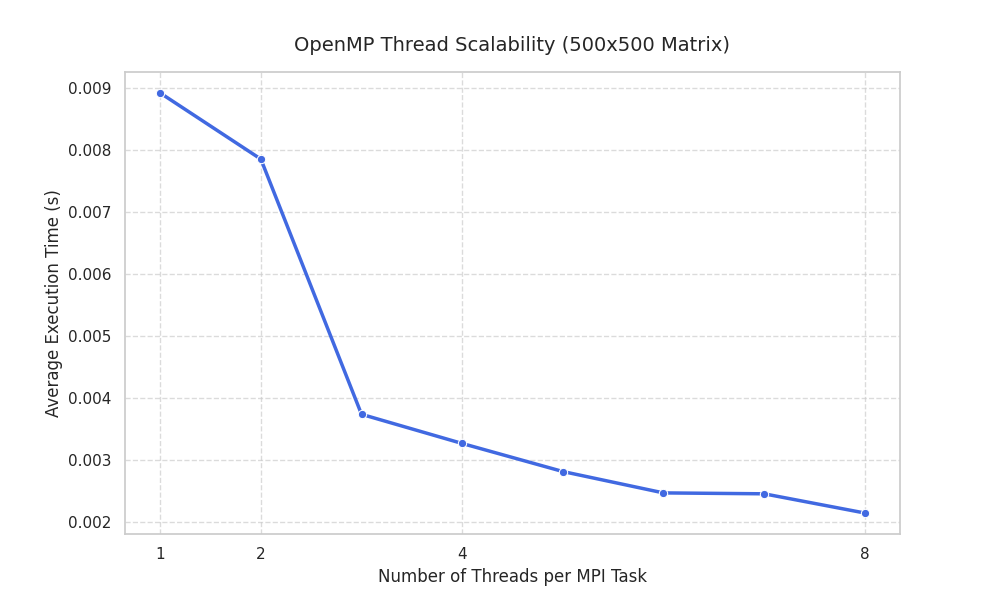
\includegraphics[width=0.85\linewidth]{MPI/thread_scalability_500.png}
    \caption{Average execution time as a function of threads per MPI task ($500 \times 500$ matrix).}
    \label{fig:thread_scalability}
\end{figure}

As shown in Figure \ref{fig:thread_scalability}, the performance generally follows the trend predicted by Amdahl's Law: increasing the number of threads reduces the execution time until a plateau is reached (around 6-8 threads). However, a significant anomaly is observed in the transition from **2 to 3 threads**, where the execution time drops abruptly from $\sim 0.0078$s to $\sim 0.0037$s—a reduction of over $50\%$ for only a $33\%$ increase in raw processing units.

This "jump" suggests a transition from a software-bound bottleneck to a hardware-optimized state. In the context of the **Intel Xeon Sapphire Rapids** architecture, this behavior can be attributed to:
\begin{itemize}
    \item \textbf{Cache Locality and Tiling}: Sapphire Rapids utilizes a multi-die (tile-based) architecture. With 5 threads, the sub-blocks of the $500 \times 500$ matrix might reach an optimal size that fits entirely within the L2 or L3 cache slices associated with the active cores, drastically reducing memory latency.
    \item \textbf{Memory Controllers and Bandwidth}: The transition to 5 threads may trigger a more efficient use of the integrated Memory Controllers (iMCs), especially if the workload distribution better aligns with the mesh interconnect topology of the Sapphire Rapids socket.
    \item \textbf{AVX-512 and AMX Utilization}: If the implementation utilizes Intel Advanced Matrix Extensions (AMX), the 5-thread configuration might reach the critical threshold for hardware acceleration that was underutilized with only 2 threads.
\end{itemize}

\subsection*{Matrix Dimension Scalability}

\begin{figure}[htbp]
    \centering
    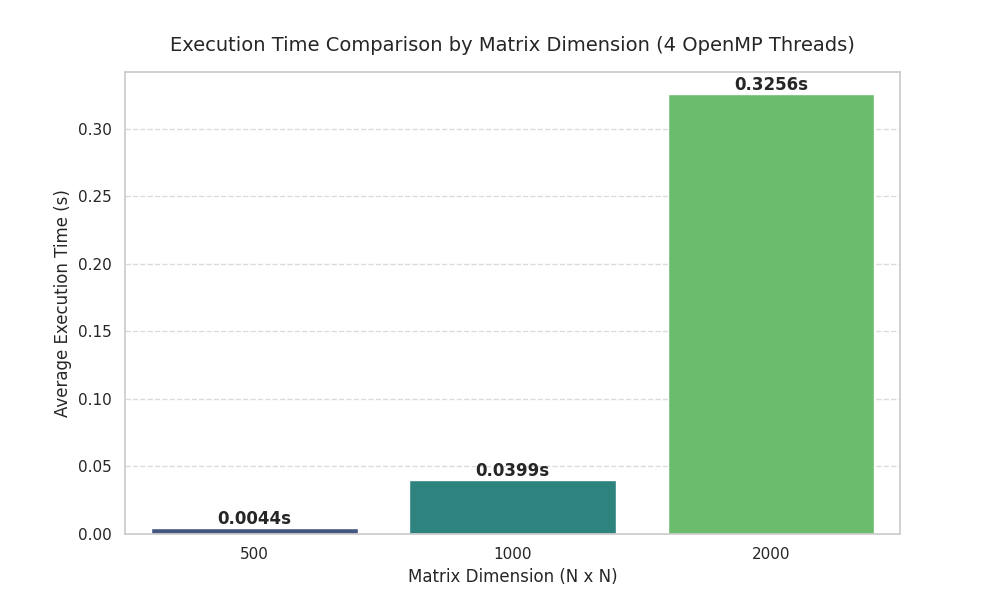
\includegraphics[width=0.85\linewidth]{MPI/matrix_dimension_comparison.png}
    \caption{Execution time comparison across different matrix dimensions ($N \times N$) using 4 OpenMP threads.}
    \label{fig:matrix_comparison}
\end{figure}

Figure \ref{fig:matrix_comparison} illustrates how the system handles increasing workloads. Matrix multiplication follows a theoretical complexity of $O(N^3)$. Our empirical data aligns closely with this:
\begin{itemize}
    \item Moving from $N=500$ ($0.0044$s) to $N=1000$ ($0.0399$s) results in an increase of factor $\approx 9.06 \times$.
    \item Moving from $N=1000$ to $N=2000$ ($0.3256$s) results in an increase of factor $\approx 8.16 \times$.
\end{itemize}
The theoretical scaling factor for doubling $N$ is $2^3 = 8$. The slight overhead observed at $N=1000$ is likely due to the increased communication volume in Cannon's algorithm, as the MPI message sizes for sub-block swaps grow quadratically ($N^2$) with the matrix dimension.

\section{CUDA}
\section*{Introduction}
This exercise requires the application of a convolutional filter to a series of images characterized by the following variables:
\begin{itemize}
    \item \textbf{Resolution:} 4K, 8K, and 16K
    \item \textbf{Noise level:} 50\%, 75\%, and 90\%
\end{itemize}
The filter must also be applied to a noiseless (ground truth) image to verify its baseline behavior, resulting in a total of 12 different image files processed during each testing iteration.

\section*{Methodology and Architecture Optimization}

\subsection*{Filter Implementation and Algorithmic Approach}
The application requires the execution of a 2D stencil operation to process multi-dimensional data. The baseline operation consists of applying a specific $3\times3$ weighted average filter, denoted as $W$, to mitigate image noise. 

The mathematical model relies on a discrete 2D spatial convolution, where each output pixel $g(x,y)$ is computed by convolving the input image $f$ with the static kernel $W$. To maximize throughput on the SIMT (Single Instruction, Multiple Threads) architecture of the NVIDIA GPU, the algorithm processes the three RGB color channels concurrently by allocating separate device memory buffers and executing the convolution kernels iteratively over the image grid.

\section*{Resolution Strategy}
\subsection*{GPU Memory Hierarchy: Tiling and Shared Memory}
A naive implementation of a $3\times3$ 2D convolution requires 9 global memory reads and 1 global memory write per pixel. For a 16K resolution image ($15360 \times 8640$ pixels per channel), this approach severely bottlenecks the execution, leaving the Streaming Multiprocessors (SMs) starved for data due to global memory latency and low bus utilization. 

To overcome this memory-bound limitation, a Tiling strategy utilizing Shared Memory was implemented. The image is divided into 2D blocks (tiles) matching the thread block dimensions (e.g., $16\times16$ or $32\times32$). Each thread block collaboratively loads its corresponding tile from the high-latency Global Memory into the ultra-fast, on-chip Shared Memory. To correctly compute the convolution at the tile boundaries without redundant fetches, the shared memory allocation includes a 1-pixel wide \textit{Halo} (or \textit{Ghost Zone}), as detailed in Listing \ref{lst:shared_mem}. 

\begin{lstlisting}[style=cppstyle, caption={Shared memory allocation and collaborative fetching of the Halo region.}, label={lst:shared_mem}]
// Allocation: block dimensions (e.g., 32x32) + 2 pixels for the Halo
__shared__ unsigned char s_data[34][34];

// Fetch of the central pixel mapped to the thread
s_data[ty + 1][tx + 1] = input[g_y * width + g_x];

// Collaborative fetch of boundary pixels (Halo) by perimeter threads
if (tx == 0)      s_data[ty + 1][0]      = input[g_y * width + min(max(x - 1, 0), width - 1)];
if (tx == bw - 1) s_data[ty + 1][bw + 1] = input[g_y * width + min(max(x + 1, 0), width - 1)];
if (ty == 0)      s_data[0][tx + 1]      = input[min(max(y - 1, 0), height - 1) * width + g_x];
if (ty == bh - 1) s_data[bh + 1][tx + 1] = input[min(max(y + 1, 0), height - 1) * width + g_x];

// Essential synchronization barrier before mathematical computation
__syncthreads();
\end{lstlisting}

Following the \texttt{\_\_syncthreads()} barrier to ensure memory consistency, the convolution math is executed entirely out of the L1/Shared Memory space, reducing global memory accesses. It guarantees that all collaborative fetches are completed and the Shared Memory buffer is fully populated before any thread begins the convolution math, preventing race conditions and corrupted pixel reads.

\subsection*{Constant Memory for Stencil Weights}
The stencil elements of filter $W$ are fixed and identical for every thread in the computational grid. Allocating these 9 floating-point values in standard global memory or passing them dynamically would waste precious registers or cache lines. 

Instead, the matrix $W$ was declared in Constant Memory (\texttt{\_\_constant\_\_}), as shown in Listing \ref{lst:const_mem}. Constant memory is highly optimized for broadcast operations: when all threads in a Warp read the same memory address simultaneously, the constant cache serves the data in a single clock cycle, virtually eliminating the latency of weight retrieval during the Fused Multiply-Add (FMA) pipeline.

\begin{lstlisting}[style=cppstyle, caption={Filter weights statically allocated in GPU Constant Memory.}, label={lst:const_mem}]
__constant__ float d_W[9] = {
    1.0f/16.0f, 2.0f/16.0f, 1.0f/16.0f,
    2.0f/16.0f, 4.0f/16.0f, 2.0f/16.0f,
    1.0f/16.0f, 2.0f/16.0f, 1.0f/16.0f
};
\end{lstlisting}

\subsection*{Instruction-Level Parallelism and Loop Unrolling}
To further maximize the Arithmetic Logic Unit (ALU) utilization and minimize control-flow overhead a hardcoded $3\times3$ execution path was chosen. The nested \texttt{for} loops traditionally used to iterate over the kernel coordinates were aggressively flattened using Loop Unrolling, as demonstrated in Listing \ref{lst:unroll}. This optimization completely eliminates branch divergence and loop counter increments. Consequently, the CUDA cores remain fully operational without suffering instruction stalls, translating the mathematical convolution into a pure, uninterrupted arithmetic pipeline. 

\begin{lstlisting}[style=cppstyle, caption={Explicit loop unrolling for the 3x3 convolution kernel.}, label={lst:unroll}]
if (x < width && y < height) {
    float sum = 0.0f;
    // Hardcoded Fused Multiply-Add (FMA) instructions, avoiding conditional branches
    sum += s_data[ty][tx]     * d_W[0]; sum += s_data[ty][tx+1]   * d_W[1]; sum += s_data[ty][tx+2]   * d_W[2];
    sum += s_data[ty+1][tx]   * d_W[3]; sum += s_data[ty+1][tx+1] * d_W[4]; sum += s_data[ty+1][tx+2] * d_W[5];
    sum += s_data[ty+2][tx]   * d_W[6]; sum += s_data[ty+2][tx+1] * d_W[7]; sum += s_data[ty+2][tx+2] * d_W[8];
    
    output[y * width + x] = static_cast<unsigned char>(sum);
}
\end{lstlisting}


\section*{Experimental Results and Signal Analysis}

\subsection*{Execution Performance and Hardware Determinism}
Execution times were gathered across multiple runs for 4K, 8K, and 16K images using varying block sizes (Figure \ref{fig:block_size_impact_1}). The empirical data highlights the deterministic nature of the GPU hardware. For instance, processing a 16K image strictly required an average of $76.48$~ms (with a $32\times32$ block size) on a single A100 GPU, regardless of the noise density applied to the input (ranging from $0\%$ to $90\%$), as depicted in Figure \ref{fig:simd_determinism_1}. 

This consistency is a direct consequence of the SIMT execution model. Unlike a CPU, which might employ branch prediction algorithms that vary execution time based on the data payload, the CUDA cores execute the exact same number of fetch and floating-point operations for every pixel. Since the linear convolution does not contain conditional branches dependent on pixel intensity, the computational load remains perfectly constant, demonstrating absolute hardware determinism and immunity to data-dependent execution jitter.

\subsection*{Hardware Scalability and Memory Bandwidth}
To further investigate the architectural constraints, a comparative benchmark was conducted between a datacenter accelerator (NVIDIA A100, HBM2 memory) and a consumer-grade GPU (NVIDIA RTX 2060 Mobile, GDDR6 memory). The relative speed-up $S$ achieved by scaling the hardware is mathematically defined by Amdahl's framework as:
$$ S = \frac{T_{\text{baseline}}}{T_{\text{target}}} $$

The execution on the RTX 2060 (GDDR6 @ 336 GB/s) required an average of $220$~ms for a 16K resolution image, compared to the $76.48$~ms achieved by the A100 (HBM2 @ 1555 GB/s). The ratio between the execution times ($\sim2.8\times$) scales in a directly proportional manner to the ratio of their theoretical memory bandwidths ($\sim4.6\times$). This correlation, supported by the data in Table \ref{tab:hw_scalability} and Figure \ref{fig:Comparison_1}, definitively confirms the Memory-Bound nature of the 2D spatial convolution: the computational throughput is severely limited by the memory fetch latency, preventing the CUDA cores from saturating their Arithmetic Logic Unit (ALU) capacity. Similarly, a crucial finding in the multi-GPU analysis is the observation of a negative speedup ($S < 1$) when scaling from one to three A100 gpus. The arithmetic intensity is relatively low; consequently, the time saved by distributing pixels across multiple SMs is completely offset by the overhead of partitioning the image buffer, managing memory copies via the PCIe/NVLink bus, and synchronizing the sub-tiles for the final composition.

\section*{Obtained Data}
\subsection*{PSNR Degradation: Failure of Linear Filtering on Impulse Noise}
The effectiveness of the assigned $W$ filter was quantitatively evaluated using the Peak Signal-to-Noise Ratio (PSNR) metric against independent colour impulse noise (Salt-and-Pepper). The experimental results (Figure \ref{fig:psnr_degradation_1}) demonstrate a catastrophic collapse of the PSNR as the noise density increases. For 16K images, the baseline PSNR drops from $36.18$~dB (clean image) down to $15.97$~dB at $90\%$ noise density, completely compromising the visual information.
% NOTA: Richiede il pacchetto \usepackage{booktabs} nel preambolo
\begin{table}[h!]
    \centering
    \caption{Hardware Scalability Analysis: Mean Execution Time, Variance, and Relative Speedup (Block Size $32\times32$)}
    \label{tab:hw_scalability}
    \begin{tabular}{lccc}
        \toprule
        \textbf{Hardware} & \textbf{Mean Time (ms)} & \textbf{Variance (ms$^2$)} & \textbf{Speedup} \\
        \midrule
        \multicolumn{4}{c}{\textbf{Resolution: 4K}} \\
        \midrule
        RTX 2060 Mobile & 16.05 & 0.37 & 0.67$\times$ \\
        1 A100 & 10.75 & 1.89 & 1.00$\times$ \\
        2 A100 & 21.66 & 64.57 & 0.50$\times$ \\
        3 A100 & 14.37 & 8.90 & 0.75$\times$ \\
        \midrule
        \multicolumn{4}{c}{\textbf{Resolution: 8K}} \\
        \midrule
        RTX 2060 Mobile & 62.42 & 92.13 & 0.46$\times$ \\
        1 A100 & 28.87 & 277.02 & 1.00$\times$ \\
        2 A100 & 29.82 & 51.59 & 0.97$\times$ \\
        3 A100 & 26.21 & 7.98 & 1.10$\times$ \\
        \midrule
        \multicolumn{4}{c}{\textbf{Resolution: 16K}} \\
        \midrule
        RTX 2060 Mobile & 220.32 & 42.80 & 0.35$\times$ \\
        1 A100 & 76.48 & 2.44 & 1.00$\times$ \\
        2 A100 & 82.82 & 46.29 & 0.92$\times$ \\
        3 A100 & 82.52 & 52.29 & 0.93$\times$ \\
        \bottomrule
    \end{tabular}
\end{table}


From a signal processing perspective, this behaviour is mathematically expected. The filter $W$ acts as a low-pass spatial filter (a weighted local average). Impulse noise introduces extremely high spatial frequencies, mathematically modelled as Dirac delta functions in the spatial domain. A linear operator like filter $W$ cannot reject these impulses; it merely computes their convolution, effectively distributing the noise energy over the adjacent pixels within its $3\times3$ support region. Consequently, the high-amplitude noise is not eliminated but rather spatially smeared, resulting in a blurred image with pervasive chromatic aberrations. 

This analysis strictly validates that while linear low-pass filters are effective against Gaussian noise, non-linear filters (such as the Median filter) are mandatory to successfully process the images and get a satisfactory result.

%\clearpage
\section*{Appendix: Figures and Data Tables}

% Grafico 1: Block Size Impact
\begin{figure}[htbp]
    \includesvg[width=0.85\linewidth]{CUDA/Plot_1_1A100_BlockSize_Impact}
    \caption{Impact of Thread Block Size on Execution Time on a single NVIDIA A100.}
    \label{fig:block_size_impact_1}
\end{figure}

\begin{figure}[htbp]
    \centering
    \includesvg[width=0.85\linewidth]{CUDA/Plot_1_2A100_BlockSize_Impact}
    \caption{Impact of Thread Block Size on Execution Time on two NVIDIA A100}
    \label{fig:block_size_impact_2}
\end{figure}

\begin{figure}[htbp]
    \centering
    \includesvg[width=0.85\linewidth]{CUDA/Plot_1_3A100_BlockSize_Impact}
    \caption{Impact of Thread Block Size on Execution Time on three NVIDIA A100}
    \label{fig:block_size_impact_3}
\end{figure}

\begin{figure}[htbp]
    \centering
    \includesvg[width=0.85\linewidth]{CUDA/Plot_1_RTX2060_BlockSize_Impact}
    \caption{Impact of Thread Block Size on Execution Time on a RTX 2060 Mobile}
    \label{fig:block_size_impact_2060}
\end{figure}
% Grafico 2: Determinismo
\begin{figure}[htbp]
    \includesvg[width=0.85\linewidth]{CUDA/Plot_3_1A100_SIMD_Determinism.svg}
    \caption{Execution time stability across varying impulse noise densities}
    \label{fig:simd_determinism_1}
\end{figure}

\begin{figure}[htbp]
    \includesvg[width=0.85\linewidth]{CUDA/Plot_3_2A100_SIMD_Determinism.svg}
    \caption{Execution time stability across varying impulse noise densities.}
    \label{fig:simd_determinism_2}
\end{figure}

\begin{figure}[htbp]
    \includesvg[width=0.85\linewidth]{CUDA/Plot_3_3A100_SIMD_Determinism.svg}
    \caption{Execution time stability across varying impulse noise densities}
    \label{fig:simd_determinism_3}
\end{figure}

\begin{figure}[htbp]
    \includesvg[width=0.85\linewidth]{CUDA/Plot_3_RTX2060_SIMD_Determinism.svg}
    \caption{Execution time stability across varying impulse noise densities}
    \label{fig:simd_determinism_2060}
\end{figure}

% Grafico 3: Comparazione Hardware A100 vs RTX
\begin{figure}[htbp]
    \centering
    \includesvg[width=0.85\linewidth]{CUDA/Plot_4_Hardware_Comparison_BS8}
    \caption{Comparative hardware execution time scaling (RTX 2060 vs. Multi-GPU A100) [8 Blocks]}
    \label{fig:Comparison_1}
\end{figure}

\begin{figure}[htbp]
    \centering
    \includesvg[width=0.85\linewidth]{CUDA/Plot_4_Hardware_Comparison_BS16}
    \caption{Comparative hardware execution time scaling (RTX 2060 vs. Multi-GPU A100) [16 Blocks]}
    \label{fig:Comparison_2}
\end{figure}

\begin{figure}[htbp]
    \includesvg[width=0.85\linewidth]{CUDA/Plot_4_Hardware_Comparison_BS32}
    \caption{Comparative hardware execution time scaling (RTX 2060 vs. Multi-GPU A100) [32 Blocks]}
    \label{fig:Comparison_3}
\end{figure}

% Grafico 4: PSNR Degradation
\begin{figure}[htbp]
    \centering
    \includesvg[width=0.85\linewidth]{CUDA/Plot_2_1A100_PSNR_Degradation.svg}
    \caption{PSNR degradation of the linear $3\times3$ filter when subjected to high-density impulse noise.}
    \label{fig:psnr_degradation_1}
\end{figure}

\begin{figure}[htbp]
    \centering
    \includesvg[width=0.85\linewidth]{CUDA/Plot_2_2A100_PSNR_Degradation.svg}
    \caption{PSNR degradation of the linear $3\times3$ filter when subjected to high-density impulse noise.}
    \label{fig:psnr_degradation_2}
\end{figure}

\begin{figure}[htbp]
    \centering
    \includesvg[width=0.85\linewidth]{CUDA/Plot_2_3A100_PSNR_Degradation.svg}
    \caption{PSNR degradation of the linear $3\times3$ filter when subjected to high-density impulse noise.}
    \label{fig:psnr_degradation_3}
\end{figure}

\begin{figure}[htbp]
    \centering
    \includesvg[width=0.85\linewidth]{CUDA/Plot_2_RTX2060_PSNR_Degradation.svg}
    \caption{PSNR degradation of the linear $3\times3$ filter when subjected to high-density impulse noise.}
    \label{fig:psnr_degradation_2060}
\end{figure}


\clearpage
\newpage
\section{OPEN MP}
\section*{Introduction}
This exercise involves developing a program using OpenMP to simulate heat diffusion across a metal plate, represented as a 1024×1024 grid of blocks. Each block is initialized with a specified initial temperature, and the program models how heat propagates through the grid over time. Two different initial conditions are examined, with particular attention given to the simulation process, computational cost, and execution time. Special focus is put on analysing how the number of threads affects performance. The simulation is carried out several times for different amounts of iterations up to 10,000 to evaluate efficiency and the effect of the increase of the number of threads. The simulation stops either when the number of performed iterations reaches the maximum chosen value or when the maximum change in temperature through the system does not exceed a chosen threshold value $ABS\_EPS$.

\section*{Resolution Strategy}
The approach to solving the exercise was to create two 1024×1024 matrices. One matrix stores the current temperatures of the grid, while the other is updated during each iteration with the results of the diffusion process. After every iteration, the roles of the matrices are swapped: the updated matrix becomes the new current state, and the other is reused as the output matrix for the next iteration.\\
For each cell two possible cases are considered:
\begin{itemize}
\item \textbf{Border}: cells located on the boundary of the matrix. A cell is classified as a border cell if either of its coordinates, x or y, is equal to 0 or 1023.
\item \textbf{Internal}: all remaining cells, which are fully surrounded by other cells within the metal plate.
\end{itemize}
The updated temperature value for each internal cell is computed according to the following scheme:\\
\(Out[i][j] = coeff * In[i][j] + W_x * (In[i][j - 1)\)\\ \(+ In[i][j + 1]) + W_y * (In[i - 1][j] + In[i + 1][j]);\)\\
Here, the values in In correspond to the temperature from the previous iteration, while \(W_x\) and \(W_y\) represent material conductivity coefficients in the \(x\) and \(y\) directions, respectively.
The coefficient for each cell is given by:
\(coeff = 1.0f - 2.0f * (Wx + Wy);\)
For all simulations the parameters are set to $W_x=0.2$ and $W_y=0.3$ .
In the case of a border cell the formula is changed to consider a lower number of neighbouring cells.

Regarding the distribution of the cells across the different threads, the following directive was utilized: 
\begin{lstlisting}[style=cppstyle]
    #pragma omp parallel for collapse(2)
\end{lstlisting}
This approach divides the cells over both rows and columns. Given that the simulation consists of $1024 \times 1024$ input cells, which corresponds to $1{,}048{,}576$ total cells, each thread is assigned a number of cells equal to:
$$N_{cells} = \frac{N_{cells-TOT}}{N_{threads}}$$
These cells are contiguous due to the implementation of the default static scheduling. This specific scheduling strategy was selected because all operations performed on the cells require approximately the same amount of computational time.


\section*{Obtained data}
Multiple simulations of the diffusion problem were conducted, varying the number of threads utilized for parallel execution. Specifically, six simulations were performed using 1, 2, 4, 8, 16, and 32 threads to evaluate how execution time scales with increasing parallelism. 

Furthermore, this set of simulations was repeated across different maximum iteration counts: $1{,}000$, $2{,}000$, $3{,}000$, $5{,}000$, and $10{,}000$ iterations. Each configuration was executed 10 times to determine an average runtime and to compute the corresponding standard deviation.


To analyze the diffusion process throughout the simulation, a snapshot of the temperature distribution across the slab was recorded every $1{,}000$ iterations. These snapshots facilitated the tracking of temperature evolution over time. To avoid impacting the execution time measurements, the snapshot generation was isolated within a separate \texttt{for} loop, distinct from the loops responsible for calculating the elapsed time.

Furthermore, a Python script was developed to visualize the results. This program processes the saved snapshots to generate images wherein temperature values are mapped to varying intensities of red, thereby providing a clear visual representation of the diffusion process.
\subsection{Simulation 1}
In Simulation 1, the slab is initialized such that one half is set to a temperature of $250^{\circ}$C, while the remaining half is set to Earth's average temperature, which is approximated as $14.98^{\circ}$C.
Figure III.1 shows the evolution over time of the temperature in the slab. 
\begin{figure}[h!]
\centering
\begin{subfigure}[b]{0.15\textwidth}
    \centering
    
\includegraphics[width=\textwidth]{OPEN_MP/0-1.png}
    \caption{0 iterations}
\end{subfigure}
\hfill
\begin{subfigure}[b]{0.15\textwidth}
    \centering
    
\includegraphics[width=\textwidth]{OPEN_MP/300.png}
    \caption{3000 iterations}
\end{subfigure}

\begin{subfigure}[b]{0.15\textwidth}
    \centering
    
\includegraphics[width=\textwidth]{OPEN_MP/600.png}
    \caption{6000 iterations}
\end{subfigure}
\hfill
\begin{subfigure}[b]{0.15\textwidth}
    \centering
    
\includegraphics[width=\textwidth]{OPEN_MP/900.png}
    \caption{9000 iterations}
\end{subfigure}
\caption{Diffusion through iterations-simulation 1}
\end{figure}

As can be observed, the evolution is extremely slow through the iterations, and the temperature equilibrium is far from being reached. Moreover, the chosen threshold of 0.001 for the minimum change in the system between successive iterations was never reached, even after 10,000 iterations. To determine the number of iterations required for the simulation to terminate due to the threshold condition, the maximum iteration count was increased to $30{,}000$. The results demonstrated that the threshold was reached after $29{,}275$ iterations. \\
\begin{table}[h!]
\centering
\resizebox{\linewidth}{!}{%
\begin{tabular}{l c c c c}
\hline
Iteration Group & Threads & Mean (s) & Std Dev (s) & Speedup vs half threads \\
\hline
1000 iterations & 1  & 1.8422 & 0.0140 & - \\
1000 iterations & 2  & 0.9083 & 0.0065 & 2.03 \\
1000 iterations & 4  & 0.4708 & 0.0095 & 1.93 \\
1000 iterations & 8  & 0.4730 & 0.0008 & 0.99 \\
1000 iterations & 16 & 0.5758 & 0.0031 & 0.82 \\
1000 iterations & 32 & 0.6096 & 0.0018 & 0.94 \\
2000 iterations & 1  & 3.6575 & 0.0233 & - \\
2000 iterations & 2  & 1.8111 & 0.0063 & 2.02 \\
2000 iterations & 4  & 0.9279 & 0.0151 & 1.95 \\
2000 iterations & 8  & 0.9465 & 0.0017 & 0.98 \\
2000 iterations & 16 & 1.1493 & 0.0050 & 0.82 \\
2000 iterations & 32 & 1.2168 & 0.0025 & 0.94 \\
3000 iterations & 1  & 5.4772 & 0.0134 & - \\
3000 iterations & 2  & 2.7115 & 0.0112 & 2.02 \\
3000 iterations & 4  & 1.4007 & 0.0143 & 1.94 \\
3000 iterations & 8  & 1.4182 & 0.0013 & 0.99 \\
3000 iterations & 16 & 1.7298 & 0.0080 & 0.82 \\
3000 iterations & 32 & 1.8268 & 0.0049 & 0.95 \\
5000 iterations & 1  & 9.1473 & 0.0384 & - \\
5000 iterations & 2  & 4.5245 & 0.0161 & 2.02 \\
5000 iterations & 4  & 2.3297 & 0.0128 & 1.94 \\
5000 iterations & 8  & 2.3674 & 0.0046 & 0.98 \\
5000 iterations & 16 & 2.8671 & 0.0094 & 0.83 \\
5000 iterations & 32 & 3.0391 & 0.0078 & 0.94 \\
10000 iterations & 1  & 18.2246 & 0.0478 & - \\
10000 iterations & 2  & 9.0305  & 0.0291 & 2.02 \\
10000 iterations & 4  & 4.6693  & 0.0281 & 1.93 \\
10000 iterations & 8  & 4.7252  & 0.0022 & 0.99 \\
10000 iterations & 16 & 5.7209  & 0.0189 & 0.83 \\
10000 iterations & 32 & 6.0711  & 0.0129 & 0.94 \\
\hline
\end{tabular}%
}
\caption{Execution time performance and speed-up compared to half the number of threads- Simulation 1}
\label{tab:speedup}
\end{table}\\
As shown in Table III.1, the execution times for all simulations decrease significantly as the number of threads is increased up to 4. A speedup of approximately 2× is observed with up to 4 threads. Increasing the number of threads to 8 does not provide any significant performance improvement, while using more than 8 threads results in performance degradation. The lack of performance improvement between 4 and 8 threads suggests that, although using 8 threads provides more parallelism in the matrix calculations, it also introduces overhead due to managing additional threads. Overall, the parallel implementation demonstrates solid scalability up to eight threads, corresponding to one thread per physical core. Beyond this point, particularly when utilizing 16 or 32 threads, performance degrades. Since only 8 hardware threads are available, increasing the number of threads beyond the number of physical cores forces multiple threads to compete for the same hardware resources, introducing contention and overhead, which leads to higher execution time.\\
The same data are illustrated in Figure III.2, providing a visual representation of this trend.
\begin{figure}[htbp]
    \centering
    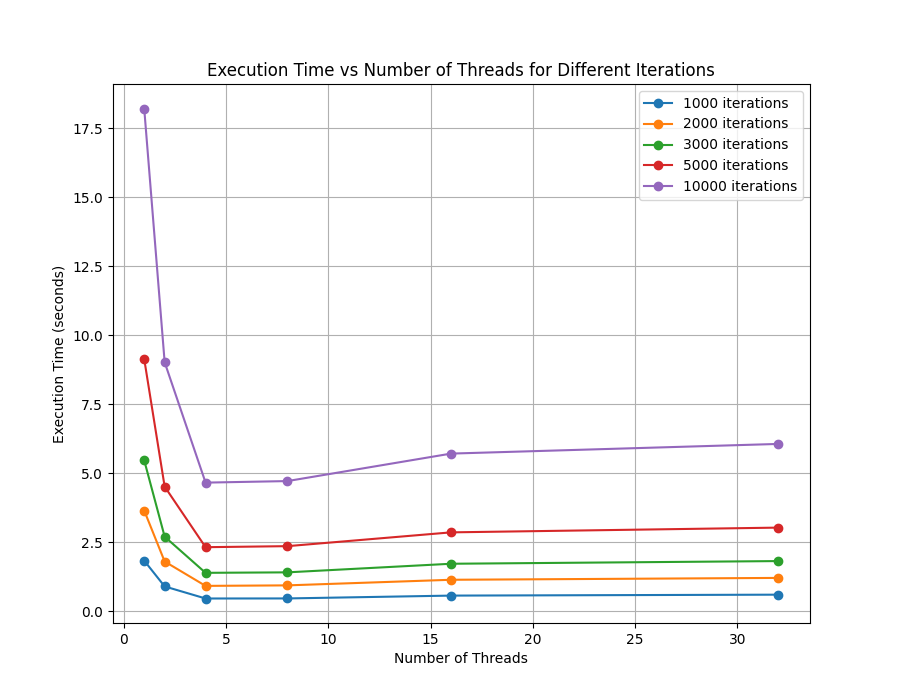
\includegraphics[width=1\linewidth]{OPEN_MP/Sim1Graph.png}
    \caption{Execution times vs Number of  threads}
    \label{fig:placeholder}
\end{figure}


The data analysis shows that the execution time increases proportionally with the number of iterations, exhibiting an almost perfectly linear relationship. This behaviour is expected, as the code performs no operations whose cost grows  with additional iterations.

\subsection{Simulation 2}
In Simulation 2, the central region of the slab, corresponding to 25\% of the total area, is initialized at a temperature of $540^{\circ}$C, while the remainder of the surface is again set to $14.98^{\circ}$C. As in the previous simulation Figure III.3 shows the evolution of the diffusion through different snapshots over time.
\begin{figure}[htbp]
\centering

\begin{subfigure}[b]{0.17\textwidth}
    \centering
    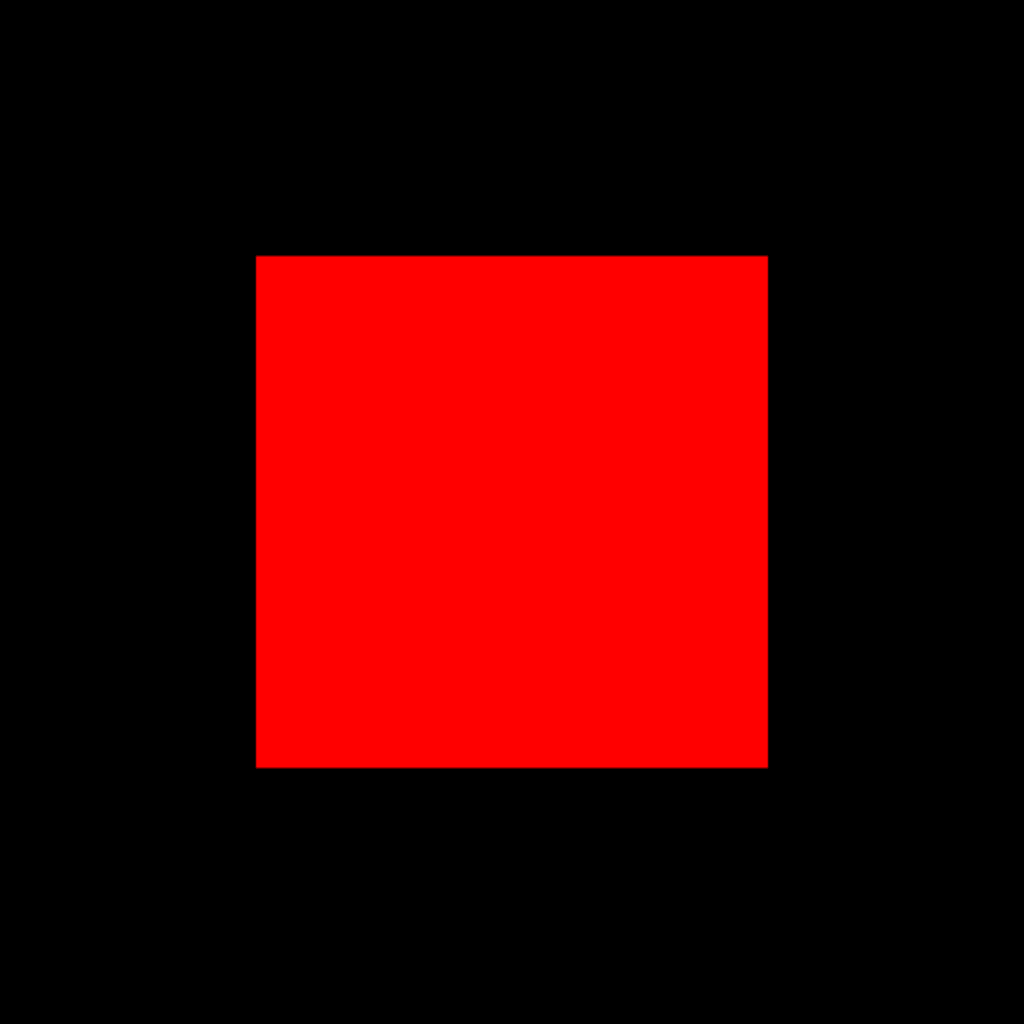
\includegraphics[width=\textwidth]{OPEN_MP/0.png}
    \caption{0 iterations}
\end{subfigure}
\hfill
\begin{subfigure}[b]{0.17\textwidth}
    \centering
    
\includegraphics[width=\textwidth]{OPEN_MP/3000.png}
    \caption{3000 iterations}
\end{subfigure}


\begin{subfigure}[b]{0.17\textwidth}
    \centering
    
\includegraphics[width=\textwidth]{OPEN_MP/6000.png}
    \caption{6000 iterations}
\end{subfigure}
\hfill
\begin{subfigure}[b]{0.17\textwidth}
    \centering
    
\includegraphics[width=\textwidth]{OPEN_MP/9000.png}
    \caption{9000 iterations}
\end{subfigure}
\caption{Diffusion through iterations}
\end{figure}
\\
A higher threshold of $0.005$ was selected compared to the previous exercise to account for the elevated temperature in the hot zone of the metal slab. This threshold was not reached within the initial $10{,}000$ iterations. By repeating the procedure from the previous simulation and extending the maximum iteration count, it was determined that the threshold was finally met at iteration $29{,}042$, at which point the simulation was terminated.

Table III.2 and Figure III.4 present the obtained data, following the format of the previous simulation. All behaviors observed in the previous simulation are reflected in these results. This includes the direct proportionality between execution time and the number of iterations, the performance improvements scaling up to 4 parallel threads, the absence of further gains with 8 threads, and the performance degradation observed when utilizing a higher number of threads.
\begin{table}[h!]
\centering
\resizebox{\linewidth}{!}{%
\begin{tabular}{l c c c c}
\hline
Iteration Group & Threads & Mean (s) & Std Dev (s) & Speedup (vs prev) \\
\hline
1000 iterations & 1  & 2.0632 & 0.1115 & - \\
1000 iterations & 2  & 1.0565 & 0.0657 & 1.95 \\
1000 iterations & 4  & 0.5571 & 0.0441 & 1.90 \\
1000 iterations & 8  & 0.5344 & 0.0371 & 1.04 \\
1000 iterations & 16 & 0.6335 & 0.0249 & 0.84 \\
1000 iterations & 32 & 0.6629 & 0.0302 & 0.96 \\
2000 iterations & 1  & 4.2163 & 0.0973 & - \\
2000 iterations & 2  & 2.0554 & 0.0811 & 2.05 \\
2000 iterations & 4  & 1.0843 & 0.0745 & 1.90 \\
2000 iterations & 8  & 1.0687 & 0.0642 & 1.01 \\
2000 iterations & 16 & 1.2816 & 0.0737 & 0.83 \\
2000 iterations & 32 & 1.3069 & 0.0492 & 0.98 \\
3000 iterations & 1  & 6.1796 & 0.2405 & - \\
3000 iterations & 2  & 3.0611 & 0.1354 & 2.02 \\
3000 iterations & 4  & 1.5846 & 0.1093 & 1.93 \\
3000 iterations & 8  & 1.5768 & 0.0775 & 1.00 \\
3000 iterations & 16 & 1.9128 & 0.0872 & 0.82 \\
3000 iterations & 32 & 1.9813 & 0.0485 & 0.97 \\
5000 iterations & 1  & 9.3821 & 0.2479 & - \\
5000 iterations & 2  & 4.6527 & 0.1391 & 2.02 \\
5000 iterations & 4  & 2.4245 & 0.0572 & 1.92 \\
5000 iterations & 8  & 2.4190 & 0.0559 & 1.00 \\
5000 iterations & 16 & 2.9354 & 0.0604 & 0.82 \\
5000 iterations & 32 & 3.1037 & 0.0649 & 0.95 \\
10000 iterations & 1  & 19.1212 & 0.1480 & - \\
10000 iterations & 2  & 9.5574  & 0.0280 & 2.00 \\
10000 iterations & 4  & 4.9451  & 0.0106 & 1.93 \\
10000 iterations & 8  & 4.9341  & 0.0085 & 1.00 \\
10000 iterations & 16 & 5.9891  & 0.0107 & 0.82 \\
10000 iterations & 32 & 6.3382  & 0.0079 & 0.94 \\
\hline
\end{tabular}%
}
\caption{Execution performance and speedup vs  thread number}
\label{tab:speedup-prev}
\end{table}

\begin{figure}[htbp]
    \centering
    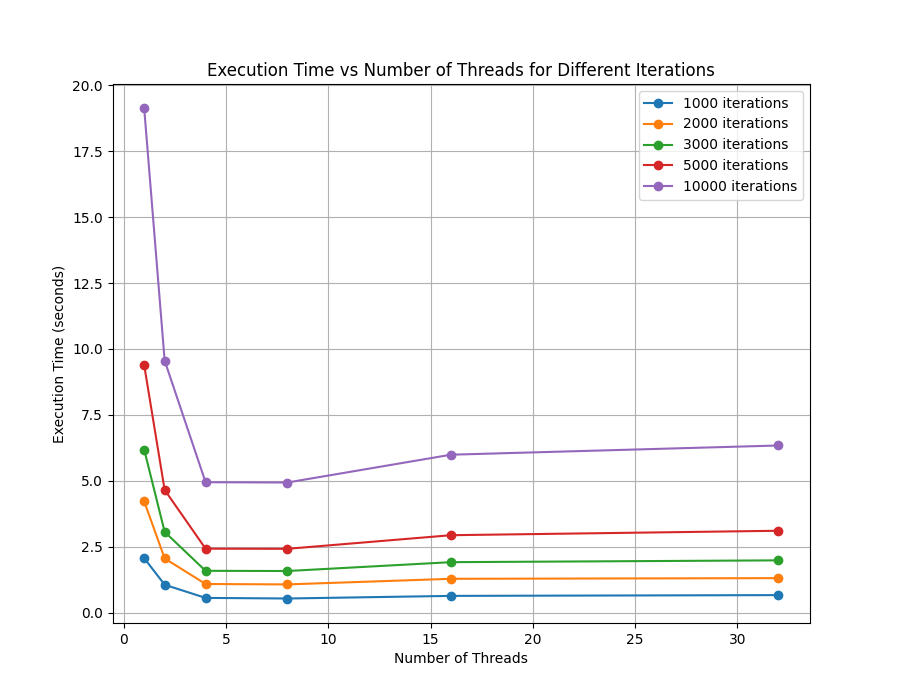
\includegraphics[width=1\linewidth]{OPEN_MP/Sim2_Graph.png}
    \caption{Execution times vs Number of  threads- Simulation 2}
    \label{fig:Sim2}
\end{figure}

\section*{CONCLUSION}
The analysis of the obtained data leads to the conclusion that the best number of threads to be chosen for these two simulations is four. In fact it is not worth for the execution times elapsed to increase further the number of used threads since it would only lead to a worsening of the performance. The model used to simulate the diffusion through the slab reaches a convergence of the diffusion increasing the number of iterations. Moreover increasing the number of simulated iterations increases proportionally the execution time for whatever number of parallel threads used. 


\begin{thebibliography}{00}
\bibitem{a1} The HPC@PoliTO Infrastructure \url{https://www.hpc.polito.it/sistemi_hpc.html}.

\end{thebibliography}



\end{document}

